% Copyright Luke Olson 2009--2014
% This work is licensed under the Creative Commons
% Attribution-NonCommercial-NoDerivatives 4.0 International License. To view a
% copy of this license, visit http://creativecommons.org/licenses/by-nc-nd/4.0/.
%
\documentclass[10pt]{beamer}
%\documentclass[handout,10pt]{beamer}
%
\mode<presentation>
{
  \usetheme[secheader]{Boadilla}
  \usecolortheme{luke}
  \usefonttheme[onlymath]{serif}
  \setbeamercovered{invisible}
  %\setbeamercovered{transparent}
  %
}
\mode<handout>
{
  \usetheme[secheader]{Boadilla}
  \usefonttheme[onlymath]{serif}
  \setbeamercovered{invisible}
  \usecolortheme{luke2}
  %\setbeamercovered{transparent}
}
\usepackage{pgf,pgfarrows,pgfnodes,pgfautomata,pgfheaps,pgfshade}
\usepackage{pxfonts}
\usepackage{pifont}
\usepackage{eulervm}
\usepackage{listings}
%\usepackage{pgfpages}
%\pgfpagesuselayout{2 on 1}[letterpaper]
%
%
%%%%%%%%%%%%%%%%%%%%%%%%%%%%%%%%%%%%%%%%%%%%%%%%%%%%%%%%%%%%%%%%%%%%%%%%


%
%
%
\newcommand{\vb}{{\bf{b}}}
\newcommand{\ve}{{\bf{e}}}
\newcommand{\vg}{{\bf{g}}}
\newcommand{\vp}{{\bf{p}}}
\newcommand{\vr}{{\bf{r}}}
\newcommand{\vu}{{\bf{u}}}
\newcommand{\vx}{{\bf{x}}}
\newcommand{\vz}{{\bf{z}}}
\newcommand{\vA}{{\bf{A}}}
\newcommand{\vU}{{\bf{U}}}
\newcommand{\mO}{{\mathcal{O}}}
\newcommand{\mF}{{\mathcal{F}}}
\definecolor{mygray}{rgb}{0.95,0.95,0.95}
\lstset{
        language=matlab,
        numbers=left, numberstyle=\tiny, stepnumber=1, numbersep=5pt,
        basicstyle=\color{black}\ttfamily\small,
        commentstyle=\color{green}\ttfamily,
        keywordstyle=\color{blue}\ttfamily,
        stringstyle=\color{red}\ttfamily,
        showstringspaces=false,
        backgroundcolor=\color{mygray},
        breaklines,
}
\newcommand{\norm}[1]{{\ensuremath{{\|#1\|}}}}
\newcommand{\matdim}[2]{\ensuremath{#1\times#2}}
\newcommand{\rank}[1]{\ensuremath{\mathrm{rank}(#1)}}
\newcommand{\epsm}{\ensuremath{\varepsilon_m}}
\newcommand{\cmd}[1]{{\normalfont\ttfamily\bfseries#1}}

\author{L. Olson}
\institute[UIUC]
{Department of Computer Science\\
University of Illinois at Urbana-Champaign\\
\vspace{0.5cm}
}
%%%%%%%%%%%%%%%%%%%%%%%%%%%%%%%%%%%%%%%%%%%%%%%%%%%%%%%%%%%%%%%%%%%%%%%%
\pgfdeclareimage[height=0.5cm]{university-logo}{./figs/uiuclogo}
\logo{\pgfuseimage{university-logo}}
%%%%%%%%%%%%%%%%%%%%%%%%%%%%%%%%%%%%%%%%%%%%%%%%%%%%%%%%%%%%%%%%%%%%%%%%
\title[CS 357]{Lecture 5}
\subtitle{Matrix, Vector Operations}
\date{September 8, 2009}

\begin{document}
% -------------------------------------------------
\begin{frame}
  \titlepage
\end{frame}
% -------------------------------------------------
% -------------------------------------------------
\begin{frame}
\frametitle{Goals:}
\begin{itemize}
  \item recall linear algebra {\tiny{ouch!}}
  \item cost analysis of basic operations
  \item identify basic solution schemes to systems
\end{itemize}
\end{frame}
% -------------------------------------------------
% -------------------------------------------------
\begin{frame}
\frametitle{Why this is important:}
\begin{itemize} 
  \item matrix problems arise in many areas of CS (information sciences,
graphics, design, etc)
  \item Basic Linear Algebra Subprograms (BLAS) is an interface standard for
operations
  \item simple systems set the stage for further development: avoiding error,
avoiding large costs
\end{itemize}
\end{frame}
%%%%%%%%%%%%%%%%%%%%%%%%%%%%%%%%%%%%%%%%%%%%%%%%%%%%%%%%%%%%%%%%%%%%%%%%
\begin{frame}
  \begin{alertblock}{Prereq}
    Linear Algebra is a prerequisite of the course!
  \end{alertblock}
  \begin{itemize}
  \item you should feel comfortable with Appendix D.1 in NMC6
  \item Appendix D.2 in NMC6 should not be a surprise
  \item look at Lecture 5a notes
  \end{itemize}
\end{frame}
%%%%%%%%%%%%%%%%%%%%%%%%%%%%%%%%%%%%%%%%%%%%%%%%%%%%%%%%%%%%%%%%%%%%%%%%
\begin{frame}
\frametitle{Matrix Inverse}

Let $A$ be a square (i.e. \matdim{n}{n}) with real elements.  The
\emph{inverse} of $A$ is designated $A^{-1}$, and has the property that
\begin{equation*}
    A^{-1}\, A = I
    \ \ \ \ \ \ \text{and} \ \ \ \ \ \
    A\, A^{-1} = I
\end{equation*}

The \textbf{formal solution} to $Ax=b$ is $x=A^{-1}b$.
\begin{align*}
              Ax &= b     \\
    A^{-1}\, A x &= A^{-1}b  \\
              Ix &= A^{-1}b   \\
               x &= A^{-1}b
\end{align*}

% ----------------------
\end{frame}
%%%%%%%%%%%%%%%%%%%%%%%%%%%%%%%%%%%%%%%%%%%%%%%%%%%%%%%%%%%%%%%%%%%%%%%%
%%%%%%%%%%%%%%%%%%%%%%%%%%%%%%%%%%%%%%%%%%%%%%%%%%%%%%%%%%%%%%%%%%%%%%%%
\begin{frame}
\frametitle{Matrix Inverse}

\begin{itemize}
\item<1-> formal solution to $Ax=b$ is $x=A^{-1}b$
\item<2-> BUT it is \emph{bad} evaluate $x$ this way
\item<3-> why?
\item<4-> we will not form $A^{-1}$, but solve for $x$ directly using
Gaussian elimination.
\end{itemize}
% ----------------------
\end{frame}
%%%%%%%%%%%%%%%%%%%%%%%%%%%%%%%%%%%%%%%%%%%%%%%%%%%%%%%%%%%%%%%%%%%%%%%%
%%%%%%%%%%%%%%%%%%%%%%%%%%%%%%%%%%%%%%%%%%%%%%%%%%%%%%%%%%%%%%%%%%%%%%%%
\begin{frame}
\frametitle{Why do we care as Numerical Analysts?}

Open questions:
\begin{itemize}
  \item How \emph{expensive} is it to solve $Ax=b$?
  \item What problems (errors) will we encounter solving $Ax=b$?
  \item Some matrices are easy/cheap to use: diagonal, tridiagonal, etc.
    \begin{itemize}
      \item are there others?  what makes something a "good" matrix
      numerically?
      \item are there bad ones?  how do we identify them numerically?
    \end{itemize}
  \item what do actual numerical analysts, engineers, developers, etc
  use?!?!
\end{itemize}

\end{frame}
%%%%%%%%%%%%%%%%%%%%%%%%%%%%%%%%%%%%%%%%%%%%%%%%%%%%%%%%%%%%%%%%%%%%%%%%
%%%%%%%%%%%%%%%%%%%%%%%%%%%%%%%%%%%%%%%%%%%%%%%%%%%%%%%%%%%%%%%%%%%%%%%%
\begin{frame}
\frametitle{Formal Solution when $A$ is \matdim{n}{n}}


The \emph{formal solution} to $Ax=b$ is
\begin{equation*}
        x = A^{-1}b
\end{equation*}
where $A$ is \matdim{n}{n}.

If $A^{-1}$ exists then $A$ is said to be \textbf{nonsingular}.

If $A^{-1}$ does not exist then $A$ is said to be \textbf{singular}.

% ----------------------
\end{frame}
%%%%%%%%%%%%%%%%%%%%%%%%%%%%%%%%%%%%%%%%%%%%%%%%%%%%%%%%%%%%%%%%%%%%%%%%
%%%%%%%%%%%%%%%%%%%%%%%%%%%%%%%%%%%%%%%%%%%%%%%%%%%%%%%%%%%%%%%%%%%%%%%%
\begin{frame}
\frametitle{Formal Solution when $A$ is \matdim{n}{n}}

If $A^{-1}$ exists then
\begin{equation*}
	Ax=b \qquad\Longrightarrow\qquad x = A^{-1}b
\end{equation*}
but

\begin{center}
%\begin{minipage}{13cm}
\begin{minipage}{0.8\textwidth}%{13cm}
    \raggedright
    \bfseries Do not compute the solution to $Ax=b$ by\newline
    finding $A^{-1}$, and then multiplying $b$ by $A^{-1}$!
%\end{minipage}
%% \end{center}
%% 
%% \begin{center}
\par\vspace{4ex}
\begin{tabular}{lp{50ex}}
  \textbf{We see:}  &  $x = A^{-1}b$  \\[12pt]
	\textbf{We do:} &
    Solve $Ax=b$ by Gaussian elimination\newline or an equivalent algorithm
\end{tabular}
\end{minipage}
\end{center}

% ----------------------
\end{frame}
%%%%%%%%%%%%%%%%%%%%%%%%%%%%%%%%%%%%%%%%%%%%%%%%%%%%%%%%%%%%%%%%%%%%%%%%
%%%%%%%%%%%%%%%%%%%%%%%%%%%%%%%%%%%%%%%%%%%%%%%%%%%%%%%%%%%%%%%%%%%%%%%%
\begin{frame}
\frametitle{Singularity of $A$}

If an \matdim{n}{n} matrix, $A$, is \textbf{singular} then
\begin{itemize}
    \item   the columns of $A$ are linearly dependent
    \item   the rows of $A$ are linearly dependent
    \item   $\rank{A}<n$
    \item   $\det(A)=0$
    \item   $A^{-1}$ does not exist
    \item   a solution to $Ax=b$ may not exist
    \item   If a solution to $Ax=b$ exists, it is not unique
\end{itemize}

% ----------------------
\end{frame}
%%%%%%%%%%%%%%%%%%%%%%%%%%%%%%%%%%%%%%%%%%%%%%%%%%%%%%%%%%%%%%%%%%%%%%%%
%%%%%%%%%%%%%%%%%%%%%%%%%%%%%%%%%%%%%%%%%%%%%%%%%%%%%%%%%%%%%%%%%%%%%%%%
\begin{frame}
\frametitle{Summary of Requirements for Solution of $Ax=b$}

Given the \matdim{n}{n} matrix $A$ and the \matdim{n}{1} vector, $b$
\begin{itemize}
    \item   the solution to $Ax=b$ exists and is unique for any $b$
            if and only if $\rank{A}=n$.
\end{itemize}

\begin{alertblock}{}
Recall: rank $=$ \# of linearly independent rows or columns
\end{alertblock}

\begin{alertblock}{}
Recall: $Range(A) =$ set of vectors $y$ such that $Ax=y$ for some $x$
\end{alertblock}


% ----------------------
\end{frame}
%%%%%%%%%%%%%%%%%%%%%%%%%%%%%%%%%%%%%%%%%%%%%%%%%%%%%%%%%%%%%%%%%%%%%%%%
%%%%%%%%%%%%%%%%%%%%%%%%%%%%%%%%%%%%%%%%%%%%%%%%%%%%%%%%%%%%%%%%%%%%%%%%
\begin{frame}
\frametitle{Solving a system}
\begin{equation*}
Ax=b
\end{equation*}
Three situations:
\begin{enumerate}
  \item $A$ is nonsingular: There exists a unique solution $x=A^{-1} b$

  \item $A$ is singular and $b \in Range(A)$: There are infinite solutions.

  \item $A$ is singular and $b \notin Range(A)$: There no solutions.
\end{enumerate}

\begin{enumerate}
  \item 
$A=\begin{bmatrix}2&0\\0&4\\\end{bmatrix}$
$b=\begin{bmatrix}1\\8\\\end{bmatrix}$, then
$x=\begin{bmatrix}1/2\\2\\\end{bmatrix}$.

  \item 
$A=\begin{bmatrix}2&0\\0&0\\\end{bmatrix}$
$b=\begin{bmatrix}1\\0\\\end{bmatrix}$, then infinitely many solutions.
$x=\begin{bmatrix}1/2\\\alpha\\\end{bmatrix}$.

  \item 
$A=\begin{bmatrix}2&0\\0&0\\\end{bmatrix}$
$b=\begin{bmatrix}1\\1\\\end{bmatrix}$, then no solutions.
\end{enumerate}


% ----------------------
\end{frame}
%%%%%%%%%%%%%%%%%%%%%%%%%%%%%%%%%%%%%%%%%%%%%%%%%%%%%%%%%%%%%%%%%%%%%%%%
%%%%%%%%%%%%%%%%%%%%%%%%%%%%%%%%%%%%%%%%%%%%%%%%%%%%%%%%%%%%%%%%%%%%%%%%
\begin{frame}
\frametitle{What's the big deal? ....cost}
Look at 1D:
\begin{itemize}
  \item 3 equations
  \item 3 unknowns
  \item each unknown coupled to its neighbor
\end{itemize}
\begin{equation*}
\begin{matrix}
2x_1 & -x_2 & & = 5.8\\
-x_1 & 2x_2 & -x_3& = 13.9\\
     & -x_2 & 2x_3& = 0.03\\
\end{matrix}
\end{equation*}
or 
\begin{equation*}
  \begin{bmatrix}
  2 & -1 & 0\\
  -1 &  2 & -1\\
  0 & -1 & 2\\
  \end{bmatrix}
  \begin{bmatrix}
  x_1\\x_2\\x_3\\
  \end{bmatrix}
  \begin{bmatrix}
  5.8\\13.9\\0.03\\
  \end{bmatrix}
\end{equation*}
\end{frame}
%%%%%%%%%%%%%%%%%%%%%%%%%%%%%%%%%%%%%%%%%%%%%%%%%%%%%%%%%%%%%%%%%%%%%%%%
\begin{frame}
\frametitle{Easy in 1d}
\begin{columns}
  \begin{column}{0.48\textwidth}
  \pgfimage[width=\textwidth]{figs/grid1}
  \end{column}
  \begin{column}{0.48\textwidth}
  \pgfimage[width=\textwidth]{figs/grid4}
  \end{column}
\end{columns}
\begin{columns}
  \begin{column}{0.48\textwidth}
  \begin{equation*}
  \begin{bmatrix}
    2&-1      &   &        &      & \\
     & \ddots &   &        &      & \\
     & -1     & 2 & -1     &      & \\
     &        &   & \ddots &      & \\
     &        &   &        & -1   & 2\\
  \end{bmatrix}
  \end{equation*}
  \end{column}
  \begin{column}{0.48\textwidth}
  \begin{itemize}
  \item $n$ points in the grid
  \item $3*(n-2)+2+2$ or about $3n$ nonzeros in the matrix
  \item trididagonal (easy)
  \end{itemize}
  \end{column}
\end{columns}
\end{frame}
%%%%%%%%%%%%%%%%%%%%%%%%%%%%%%%%%%%%%%%%%%%%%%%%%%%%%%%%%%%%%%%%%%%%%%%%
%%%%%%%%%%%%%%%%%%%%%%%%%%%%%%%%%%%%%%%%%%%%%%%%%%%%%%%%%%%%%%%%%%%%%%%%
\begin{frame}
\frametitle{2D: harder}
\begin{columns}
  \begin{column}{0.48\textwidth}
  \pgfimage[width=\textwidth]{figs/grid2}
  \end{column}
  \begin{column}{0.48\textwidth}
  \pgfimage[width=\textwidth]{figs/grid5}
  \end{column}
\end{columns}
\begin{columns}
  \begin{column}{0.48\textwidth}
  \begin{equation*}
  \begin{bmatrix}
    8&-1      &   &     -1  &      & \\
     & \ddots &   &         &      & \\
     -1& -1     & 8 & -1      & -1   & \\
     &        &   & \ddots &      & \\
     &   -1   &   &        & -1   & 8\\
  \end{bmatrix}
  \end{equation*}
  \end{column}
  \begin{column}{0.48\textwidth}
  \begin{itemize}
  \item $n$ points in one direction
  \item $n^2$ points in grid
  \item about 9 nonzeros in each row
  \item about $9n^2$ nonzeros in the matrix
  \item $n$-banded (harder...we will see)
  \end{itemize}
  \end{column}
\end{columns}
\end{frame}
%%%%%%%%%%%%%%%%%%%%%%%%%%%%%%%%%%%%%%%%%%%%%%%%%%%%%%%%%%%%%%%%%%%%%%%%
%%%%%%%%%%%%%%%%%%%%%%%%%%%%%%%%%%%%%%%%%%%%%%%%%%%%%%%%%%%%%%%%%%%%%%%%
\begin{frame}
\frametitle{3D: hardest}
\begin{columns}
  \begin{column}{0.48\textwidth}
  \pgfimage[width=\textwidth]{figs/grid3}
  \end{column}
  \begin{column}{0.48\textwidth}
  \pgfimage[width=\textwidth]{figs/grid6}
  \end{column}
\end{columns}
\begin{columns}
  \begin{column}{0.48\textwidth}
  \vspace{-0.5cm}
  \begin{itemize}
  \item $n$ points in one direction
  \item $n^3$ points in grid
  \end{itemize}
  \end{column}
  \begin{column}{0.48\textwidth}
  \vspace{-0.5cm}
  \begin{itemize}
  \item about 27 nonzeros in each row
  \item about $27n^3$ nonzeros in the matrix
  \item $n^2$-banded (yikes!)
  \end{itemize}
  \end{column}
\end{columns}
\end{frame}
%%%%%%%%%%%%%%%%%%%%%%%%%%%%%%%%%%%%%%%%%%%%%%%%%%%%%%%%%%%%%%%%%%%%%%%%
%%%%%%%%%%%%%%%%%%%%%%%%%%%%%%%%%%%%%%%%%%%%%%%%%%%%%%%%%%%%%%%%%%%%%%%%
\begin{frame}
\frametitle{Applications get harder and harder...}
\begin{columns}
  \begin{column}{0.48\textwidth}
  \pgfimage[height=3cm]{figs/app_sub}

  {courtesy of LLNL}
  \end{column}
  \begin{column}{0.48\textwidth}
  \pgfimage[height=3cm]{figs/app_foot}

  {courtesy of TrueGrid}
  \end{column}
\end{columns}
\begin{columns}
  \begin{column}{0.48\textwidth}
  \pgfimage[height=3cm]{figs/app_chamber}

  {courtesy of Rice}
  \end{column}
  \begin{column}{0.48\textwidth}
  \pgfimage[height=3cm]{figs/app_cfd}
  
 {courtesy of Warwick U.}
  \end{column}
\end{columns}
\end{frame}
%%%%%%%%%%%%%%%%%%%%%%%%%%%%%%%%%%%%%%%%%%%%%%%%%%%%%%%%%%%%%%%%%%%%%%%%
%%%%%%%%%%%%%%%%%%%%%%%%%%%%%%%%%%%%%%%%%%%%%%%%%%%%%%%%%%%%%%%%%%%%%%%%
\begin{frame}
\frametitle{Solving is a problem...}

\begin{center}
\begin{tabular}{c c c c c c c}
dim & unknowns & storage & example (n)& & \\\hline
1D  &   $n$    &  $3n$   & 10 & 100 & 1000\\
2D  &   $n^2$  &  $9n^2$ & $10^2$ & $10^4$ & $10^6$\\
3D  &   $n^3$  &  $27n^3$& $10^3$ & $10^6$ & $10^9$\\
\end{tabular}

\pgfimage[height=6cm]{figs/solvers}
\end{center}
\end{frame}
%%%%%%%%%%%%%%%%%%%%%%%%%%%%%%%%%%%%%%%%%%%%%%%%%%%%%%%%%%%%%%%%%%%%%%%%
%%%%%%%%%%%%%%%%%%%%%%%%%%%%%%%%%%%%%%%%%%%%%%%%%%%%%%%%%%%%%%%%%%%%%%%%
\begin{frame}
\frametitle{Moore...}
\begin{center}
\pgfimage[height=0.9\textheight]{figs/moore}
\end{center}
\end{frame}
%%%%%%%%%%%%%%%%%%%%%%%%%%%%%%%%%%%%%%%%%%%%%%%%%%%%%%%%%%%%%%%%%%%%%%%%
%%%%%%%%%%%%%%%%%%%%%%%%%%%%%%%%%%%%%%%%%%%%%%%%%%%%%%%%%%%%%%%%%%%%%%%%
\begin{frame}
\frametitle{What's the problem?}
\begin{itemize}
  \item humans: milliFLOPS
  \item hand calculators: ~ 10 FLOPS
  \item desktops: a few GFLOPS ($10^9$ FLOPS)
\end{itemize}

\begin{alertblock}{}
look at the basic operations!
\end{alertblock}
\end{frame}
%%%%%%%%%%%%%%%%%%%%%%%%%%%%%%%%%%%%%%%%%%%%%%%%%%%%%%%%%%%%%%%%%%%%%%%%
\begin{frame}
\frametitle{Big-O}
How to measure the impact of $n$ on algorithmic cost?
\begin{block}{$\mO(\cdot)$}
Let $g(n)$ be a function of $n$.  Then define
\begin{equation*}
  \mO(g(n)) = \{f(n)\,|\, \exists c,n_0>0 \,:\, 0\leq f(n)\leq cg(n),\, \forall
n\geq n_0\}
\end{equation*}

That is, $f(n)\in \mO(g(n))$ if there is a constant $c$ such that $0\leq f(n)
\leq cg(n)$ is satisfied.
\end{block}
\begin{itemize}
  \item assume non-negative functions (otherwise add $| \cdot |$) to the definitions
  \item $f(n)\in\mO(g(n))$ represents an asymptotic upper bound on $f(n)$ up to a constant
  \item example: $f(n) = 3\sqrt{n} + 2\log n + 8 n + 85 n^2 \in \mO(n^2)$
\end{itemize}
\end{frame}
%%%%%%%%%%%%%%%%%%%%%%%%%%%%%%%%%%%%%%%%%%%%%%%%%%%%%%%%%%%%%%%%%%%%%%%%
%%%%%%%%%%%%%%%%%%%%%%%%%%%%%%%%%%%%%%%%%%%%%%%%%%%%%%%%%%%%%%%%%%%%%%%%
\begin{frame}
\frametitle{Big-O (Omicron)}
\framesubtitle{asymptotic upper bound}
\begin{block}{$\mO(\cdot)$}
Let $g(n)$ be a function of $n$.  Then define
\begin{equation*}
  \mO(g(n)) = \{f(n)\,|\, \exists c,n_0>0 \,:\, 0\leq f(n)\leq cg(n),\, \forall
n\geq n_0\}
\end{equation*}

That is, $f(n)\in \mO(g(n))$ if there is a constant $c$ such that $0\leq f(n)
\leq cg(n)$ is satisfied.
\end{block}
\begin{center}
  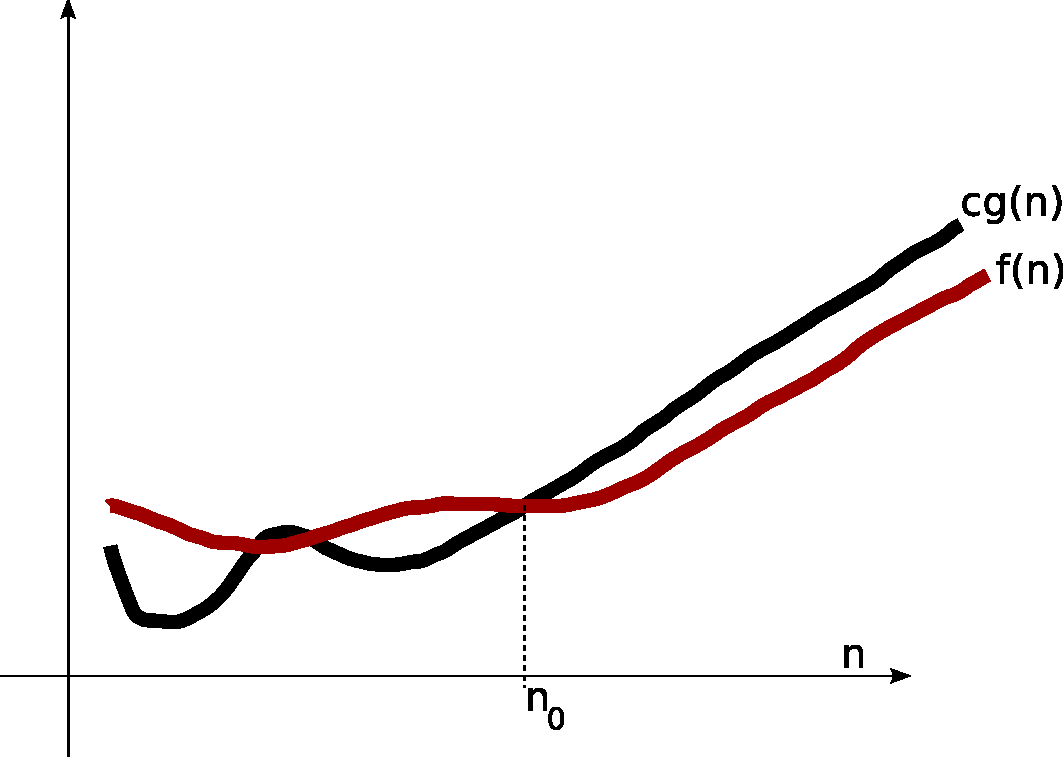
\includegraphics[height=4cm]{./figs/bigo_1}
\end{center}
\end{frame}
%%%%%%%%%%%%%%%%%%%%%%%%%%%%%%%%%%%%%%%%%%%%%%%%%%%%%%%%%%%%%%%%%%%%%%%%
%%%%%%%%%%%%%%%%%%%%%%%%%%%%%%%%%%%%%%%%%%%%%%%%%%%%%%%%%%%%%%%%%%%%%%%%
\begin{frame}
\frametitle{Big-Omega}
\framesubtitle{asymptotic lower bound}
\begin{block}{$\Omega(\cdot)$}
Let $g(n)$ be a function of $n$.  Then define
\begin{equation*}
  \Omega(g(n)) = \{f(n)\,|\, \exists c,n_0>0 \,:\, 0\leq cg(n) \leq f(n),\, \forall n\geq n_0\}
\end{equation*}

That is, $f(n)\in \Omega(g(n))$ if there is a constant $c$ such that $0\leq cg(n) \leq f(n)$ is satisfied.
\end{block}
\begin{center}
  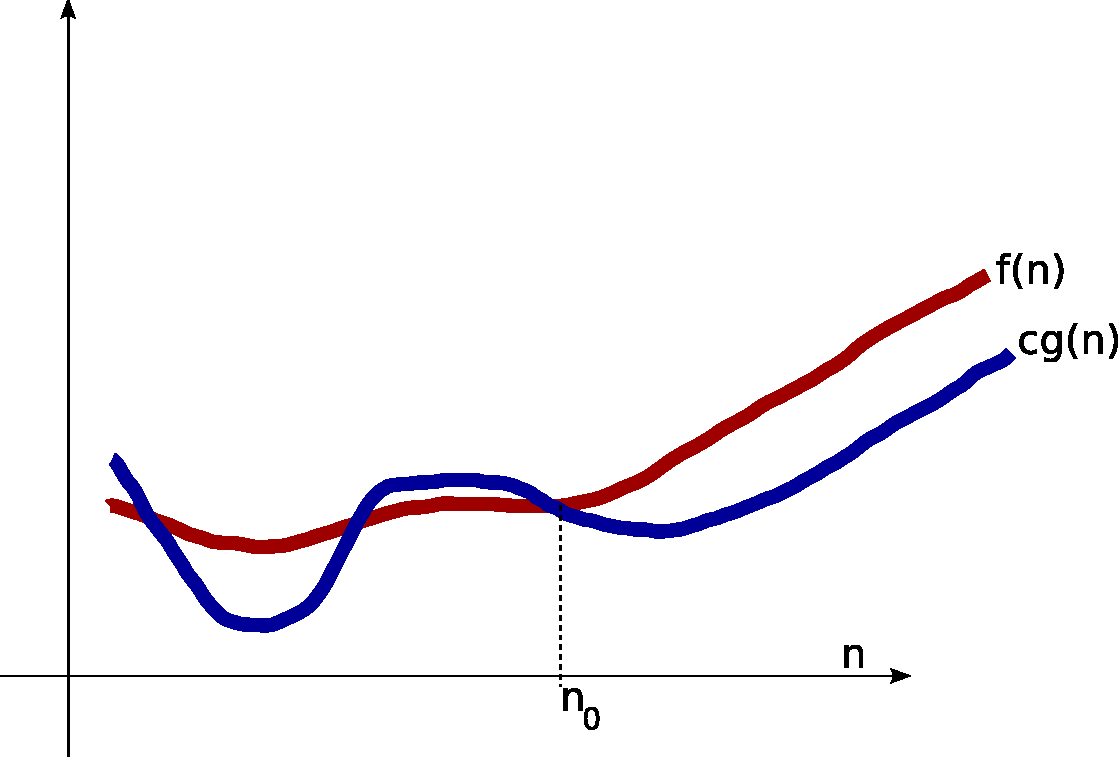
\includegraphics[height=4cm]{./figs/bigo_2}
\end{center}
\end{frame}
%%%%%%%%%%%%%%%%%%%%%%%%%%%%%%%%%%%%%%%%%%%%%%%%%%%%%%%%%%%%%%%%%%%%%%%%
%%%%%%%%%%%%%%%%%%%%%%%%%%%%%%%%%%%%%%%%%%%%%%%%%%%%%%%%%%%%%%%%%%%%%%%%
\begin{frame}
\frametitle{Big-Theta}
\framesubtitle{asymptotic tight bound}
\begin{block}{$\Theta(\cdot)$}
Let $g(n)$ be a function of $n$.  Then define
\begin{equation*}
  \Theta(g(n)) = \{f(n)\,|\, \exists c_1,c_2,n_0>0 \,:\, 0\leq c_1g(n) \leq
f(n)\leq c_2 g(n),\, \forall
n\geq n_0\}
\end{equation*}

Equivalently, $\Theta(g(n)) = \mO(g(n)) \cap \Omega(g(n))$.
\end{block}

\begin{center}
  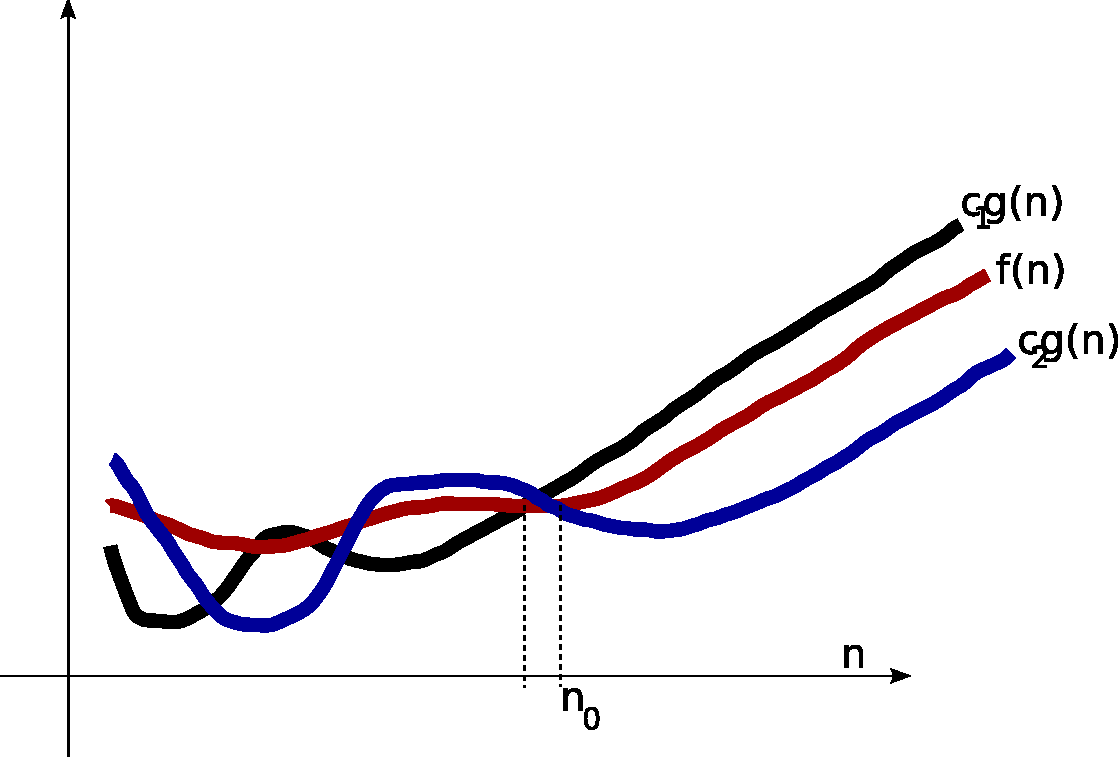
\includegraphics[height=4cm]{./figs/bigo_3}
\end{center}
\end{frame}
%%%%%%%%%%%%%%%%%%%%%%%%%%%%%%%%%%%%%%%%%%%%%%%%%%%%%%%%%%%%%%%%%%%%%%%
\begin{frame}\frametitle{BLAS}
  Basic Linear Algebra Subprograms (BLAS) interface introduced APIs for common
linear algebra tasks
  \begin{itemize}
  \item Level 1: vector operations (dot products, vector norms, etc) e.g.
    \[
    y \leftarrow \alpha x + y
\]

  \item Level 2: matrix-vector operations, e.g.
    \[
    y \leftarrow \alpha A x +  B y
\]

  \item Level 3: matrix-matrix operations, e.g.
    \[
    C \leftarrow \alpha A B +  \beta C
\]
  \item optimized versions of the reference BLAS are used everyday:  ATLAS, etc.
  \end{itemize}
\end{frame}
\begin{frame}[fragile]
\frametitle{vec-vec, mat-vec, mat-mat}
\begin{itemize}
  \item inner product of $u$ and $v$ both $[n \times 1]$
  \begin{equation*}
    \sigma  = u^T v = u_1 v_1 + \dots + u_n v_n
  \end{equation*}
  \item $\rightarrow$ $n$ multiplies, $n-1$ additions
  \item $\rightarrow$ $\mO(n)$ flops
\end{itemize}
\end{frame}
%%%%%%%%%%%%%%%%%%%%%%%%%%%%%%%%%%%%%%%%%%%%%%%%%%%%%%%%%%%%%%%%%%%%%%%%
%%%%%%%%%%%%%%%%%%%%%%%%%%%%%%%%%%%%%%%%%%%%%%%%%%%%%%%%%%%%%%%%%%%%%%%%
\begin{frame}[fragile]
\frametitle{vec-vec, mat-vec, mat-mat}
\begin{itemize}
  \item mat-vec of $A$ ($[n \times n]$) and $u$ ($[n \times 1]$)
  \begin{lstlisting}[mathescape]
    for $i=1,\dots,n$
      for $j=1,\dots,n$
        $v(i) = a(i,j)u(j) + v(i)$
      end
    end
  \end{lstlisting}
  \item $\rightarrow$ $n^2$ multiplies, $n^2$ additions
  \item $\rightarrow$ $\mO(n^2)$ flops
\end{itemize}
\end{frame}
%%%%%%%%%%%%%%%%%%%%%%%%%%%%%%%%%%%%%%%%%%%%%%%%%%%%%%%%%%%%%%%%%%%%%%%%
%%%%%%%%%%%%%%%%%%%%%%%%%%%%%%%%%%%%%%%%%%%%%%%%%%%%%%%%%%%%%%%%%%%%%%%%
\begin{frame}[fragile]
\frametitle{vec-vec, mat-vec, mat-mat}
\begin{itemize}
  \item mat-mat of $A$ ($[n \times n]$) and $B$ ($[n \times n]$)
  \begin{lstlisting}[mathescape]
    for $j=1,\dots,n$
      for $i=1,\dots,n$
        for $k=1,\dots,n$
          $C(k,j) = A(k,i)B(i,j)+C(k,j)$
        end
      end
    end
  \end{lstlisting}
  \item $\rightarrow$ $n^3$ multiplies, $n^3$ additions
  \item $\rightarrow$ $\mO(n^3)$ flops
\end{itemize}
\end{frame}
%%%%%%%%%%%%%%%%%%%%%%%%%%%%%%%%%%%%%%%%%%%%%%%%%%%%%%%%%%%%%%%%%%%%%%%%
%%%%%%%%%%%%%%%%%%%%%%%%%%%%%%%%%%%%%%%%%%%%%%%%%%%%%%%%%%%%%%%%%%%%%%%%
\begin{frame}
\frametitle{vec-vec, mat-vec, mat-mat}
\begin{center}
  \begin{tabular}{l c}\hline
  Operation & FLOPS \\\hline
  $u^T v$ & $\mO(n)$\\
  $Au$ & $\mO(n^2)$\\
  $AB$ & $\mO(n^3)$\\
  \end{tabular}
\end{center}
\begin{block}{matlab test}
  four tests:
    \begin{itemize}
      \item matrix-matrix multiply
      \item inner product
      \item matrix-vector multiply
      \item $n$ matrix-vector multiplies
    \end{itemize}
    order them...fastest to slowest
\end{block}
\begin{alertblock}{}
testflop.m
\end{alertblock}
\end{frame}
%%%%%%%%%%%%%%%%%%%%%%%%%%%%%%%%%%%%%%%%%%%%%%%%%%%%%%%%%%%%%%%%%%%%%%%%
\begin{frame}
\frametitle{Gaussian Elimination}

\begin{itemize}
\item   Solving Diagonal Systems
\item   Solving Triangular Systems
\item   Gaussian Elimination Without Pivoting
	\begin{itemize}
		\item   Hand Calculations
		\item   Cartoon Version
		\item   The Algorithm
	\end{itemize}
\item   Gaussian Elimination with Pivoting
	\begin{itemize}
		\item   Row or Column Interchanges, or Both
		\item   Implementation
	\end{itemize}
\item   Solving Systems with the Backslash Operator
\end{itemize}

% ----------------------
\end{frame}
%%%%%%%%%%%%%%%%%%%%%%%%%%%%%%%%%%%%%%%%%%%%%%%%%%%%%%%%%%%%%%%%%%%%%%%%
%%%%%%%%%%%%%%%%%%%%%%%%%%%%%%%%%%%%%%%%%%%%%%%%%%%%%%%%%%%%%%%%%%%%%%%%
\begin{frame}
\frametitle{Solving Diagonal Systems}

\onslide<1->{
The system defined by
\begin{equation*}
    A = \begin{bmatrix}1 & 0 & 0\\ 0 & 3 & 0\\ 0 & 0 & 5 \end{bmatrix}
    \ \ \ \ \ \ \
    b = \left[\negthickspace\begin{array}{r} -1 \\ 6 \\ -15 \end{array}\negthickspace\right]
\end{equation*}
}
\onslide<2->{
is equivalent to
\begin{equation*}
    \begin{array}{ccccr}
      x_1 &       &        &= &  -1  \\
          & 3 x_2 &        &= &   6  \\
          &       &  5 x_3 &= & -15
    \end{array}
\end{equation*}
}
\onslide<3->{
The solution is
\begin{align*}
    x_1 &= -1  &
    x_2 &= \frac{6}{3}=2 &
    x_3 &= \frac{-15}{5} = -3
\end{align*}
}


% ----------------------
\end{frame}
%%%%%%%%%%%%%%%%%%%%%%%%%%%%%%%%%%%%%%%%%%%%%%%%%%%%%%%%%%%%%%%%%%%%%%%%
%%%%%%%%%%%%%%%%%%%%%%%%%%%%%%%%%%%%%%%%%%%%%%%%%%%%%%%%%%%%%%%%%%%%%%%%
\begin{frame}[fragile]
\frametitle{Solving Diagonal Systems}

\begin{lstlisting}[mathescape,caption=Diagonal System Solution,label=algo:diagSolv]
  given $A$, $b$              
  for $i=1\ldots n$           
    $x_i = b_i/a_{i,i}$       
  end                         
\end{lstlisting}
\vspace{0.0cm}

\textbf{In Matlab:}
\begin{lstlisting}[language=matlab]
>> A = ...          %  A is a diagonal matrix
>> b = ...
>> x = b./diag(A)
\end{lstlisting}
This is the \emph{only} place where element-by-element division (\verb|./|)
has anything to do with solving linear systems of equations.

% ----------------------
\end{frame}
%%%%%%%%%%%%%%%%%%%%%%%%%%%%%%%%%%%%%%%%%%%%%%%%%%%%%%%%%%%%%%%%%%%%%%%%
\begin{frame}
\frametitle{Operations?}
\begin{block}{Try...}
Sketch out an operation count to solve a diagonal system of equations...
\end{block}
\onslide<2->{
\begin{block}{cheap!}
one division $n$ times $\longrightarrow$ $\mO(n)$ FLOPS
\end{block}
}
\end{frame}
%%%%%%%%%%%%%%%%%%%%%%%%%%%%%%%%%%%%%%%%%%%%%%%%%%%%%%%%%%%%%%%%%%%%%%%%
\begin{frame}
\frametitle{Triangular Systems}

The generic lower and upper triangular matrices are
\begin{equation*}
    L = \begin{bmatrix} l_{11} &   0    & \cdots &   0    \\
                        l_{21} & l_{22} &        &   0    \\
                        \vdots &        & \ddots & \vdots \\
                        l_{n1} &        & \cdots & l_{nn} \\
        \end{bmatrix}
\end{equation*}
and
\begin{equation*}
    U = \begin{bmatrix} u_{11} & u_{12} & \cdots & u_{1n} \\
                           0   & u_{22} &        & u_{2n}  \\
                        \vdots &        & \ddots & \vdots \\
                           0   &        & \cdots & u_{nn} \\
        \end{bmatrix}
\end{equation*}

The triangular systems
\begin{equation*}
    Ly = b \ \ \ \ \ \ \ \ \ Ux = c
\end{equation*}
are easily solved by \textbf{forward substitution} and
\textbf{backward substitution}, respectively

% ----------------------
\end{frame}
%%%%%%%%%%%%%%%%%%%%%%%%%%%%%%%%%%%%%%%%%%%%%%%%%%%%%%%%%%%%%%%%%%%%%%%%
%%%%%%%%%%%%%%%%%%%%%%%%%%%%%%%%%%%%%%%%%%%%%%%%%%%%%%%%%%%%%%%%%%%%%%%%
\begin{frame}
\frametitle{Solving Triangular Systems}

\onslide<1->{
\begin{equation*}
    A = \left[\negthickspace\begin{array}{rrr} -2 & 1 & 2 \\ 0 & 3 & -2 \\ 0 & 0 & 4\end{array}\negthickspace\right]
    \ \ \ \ \ \ \
    b = \left[\negthickspace\begin{array}{r} 9 \\ -1 \\ 8 \end{array}\negthickspace\right]
\end{equation*}
}
\onslide<2->{
is equivalent to
\begin{equation*}
    \begin{array}{rcrcrcr}
      -2 x_1 & + &   x_2  & + &  2x_3 &= &  9  \\
             &   &  3x_2  & + & -2x_3 &= & -1  \\
             &   &        &   &  4x_3 &= &  8  \\
    \end{array}
\end{equation*}
}
\onslide<3->{

Solve in backward order (last equation is solved first)
\begin{align*}
      x_3 &= \frac{8}{4} = 2
    & x_2 &= \frac{1}{3} \left( -1 + 2 x_3 \right) = \frac{3}{3} = 1
    \\
    & & x_1 &= \frac{\ \,1}{-2}\left( 9 - x_2 - 2 x_3 \right) = \frac{\ \,4}{-2} = -2
\end{align*}
}

% ----------------------
\end{frame}
%%%%%%%%%%%%%%%%%%%%%%%%%%%%%%%%%%%%%%%%%%%%%%%%%%%%%%%%%%%%%%%%%%%%%%%%
%%%%%%%%%%%%%%%%%%%%%%%%%%%%%%%%%%%%%%%%%%%%%%%%%%%%%%%%%%%%%%%%%%%%%%%%
\begin{frame}[fragile]
\frametitle{Solving Triangular Systems}

Solving for $x_1, x_2, \ldots, x_n$
for a lower triangular system is called \textbf{forward substitution}.
\begin{lstlisting}[mathescape,caption=,label=algo:forsub]
  given $L$, $b$               
  $x_1 = b_1/\ell_{11}$           
  for $i=2\ldots n$          
    $s = b_i$                  
    for $j = 1\ldots i-1$    
      $s = s - \ell_{i,j}x_j$   
    end                      
    $x_i = s/\ell_{i,i}$          
  end                          
\end{lstlisting}

\onslide<2->{
Using forward or backward substitution is sometimes referred
to as performing a \textbf{triangular solve}.
}

% ----------------------
\end{frame}
%%%%%%%%%%%%%%%%%%%%%%%%%%%%%%%%%%%%%%%%%%%%%%%%%%%%%%%%%%%%%%%%%%%%%%%%
%%%%%%%%%%%%%%%%%%%%%%%%%%%%%%%%%%%%%%%%%%%%%%%%%%%%%%%%%%%%%%%%%%%%%%%%
\begin{frame}
\frametitle{Operations?}
\begin{block}{Try...}
Sketch out an operation count to solve a triangular system of equations...
\end{block}
\onslide<2->{
\begin{block}{cheap!}
  \begin{itemize}
    \item begin in the bottom corner: 1 div
    \item row -2: 1 mult, 1 add, 1 div, or 3 FLOPS
    \item row -3: 2 mult, 2 add, 1 div, or 5 FLOPS
    \item row -4: 3 mult, 3 add, 1 div, or 7 FLOPS
    \item $\vdots$
    \item row -$j$: about $2j$ FLOPS
  \end{itemize}
  Total FLOPS? $\sum_{j=1}^{n} 2j = 2 \frac{ n(n+1)}{2}$ or $\mO(n^2)$ FLOPS
\end{block}
}
\end{frame}
%%%%%%%%%%%%%%%%%%%%%%%%%%%%%%%%%%%%%%%%%%%%%%%%%%%%%%%%%%%%%%%%%%%%%%%%
\end{document}
